\pagebreak
\section{Login}
\label{login}

Existiert bereits ein Account ist es möglich sich über die Log In View mit diesem anzumelden. Dafür 
wir die Email als auch das Passwort benötigt. Hierzu wird wie auch beim \underline{\nameref{createAccount}} eine 
simple HTML form verwendet. 

\begin{figure}[H]
    \begin{center}
      \frame{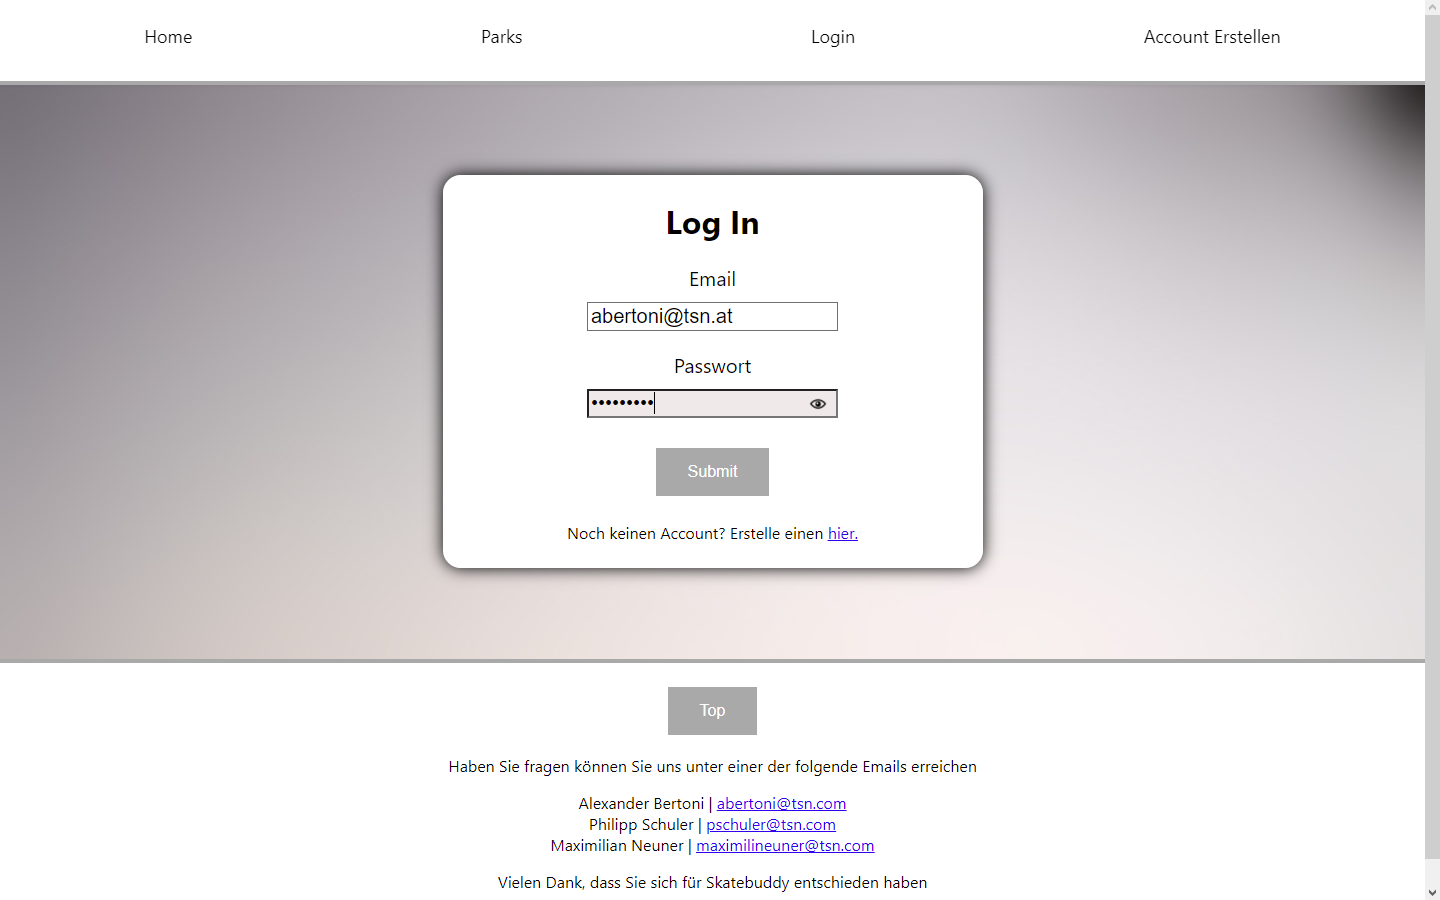
\includegraphics[width=1\textwidth]{Website/LogIn.png}}
      \caption{Login Page mit verstecktem Passwort}
    \end{center}
\end{figure}

Durch Mausklick auf das Auge in der Passworteingabe, lässt sich das Passwort für den Benutzer
anzeigen. Damit lassen sich Tippfehler beim Eingeben erkennen, falls nötig. 

\begin{figure}[H]
    \begin{center}
      \frame{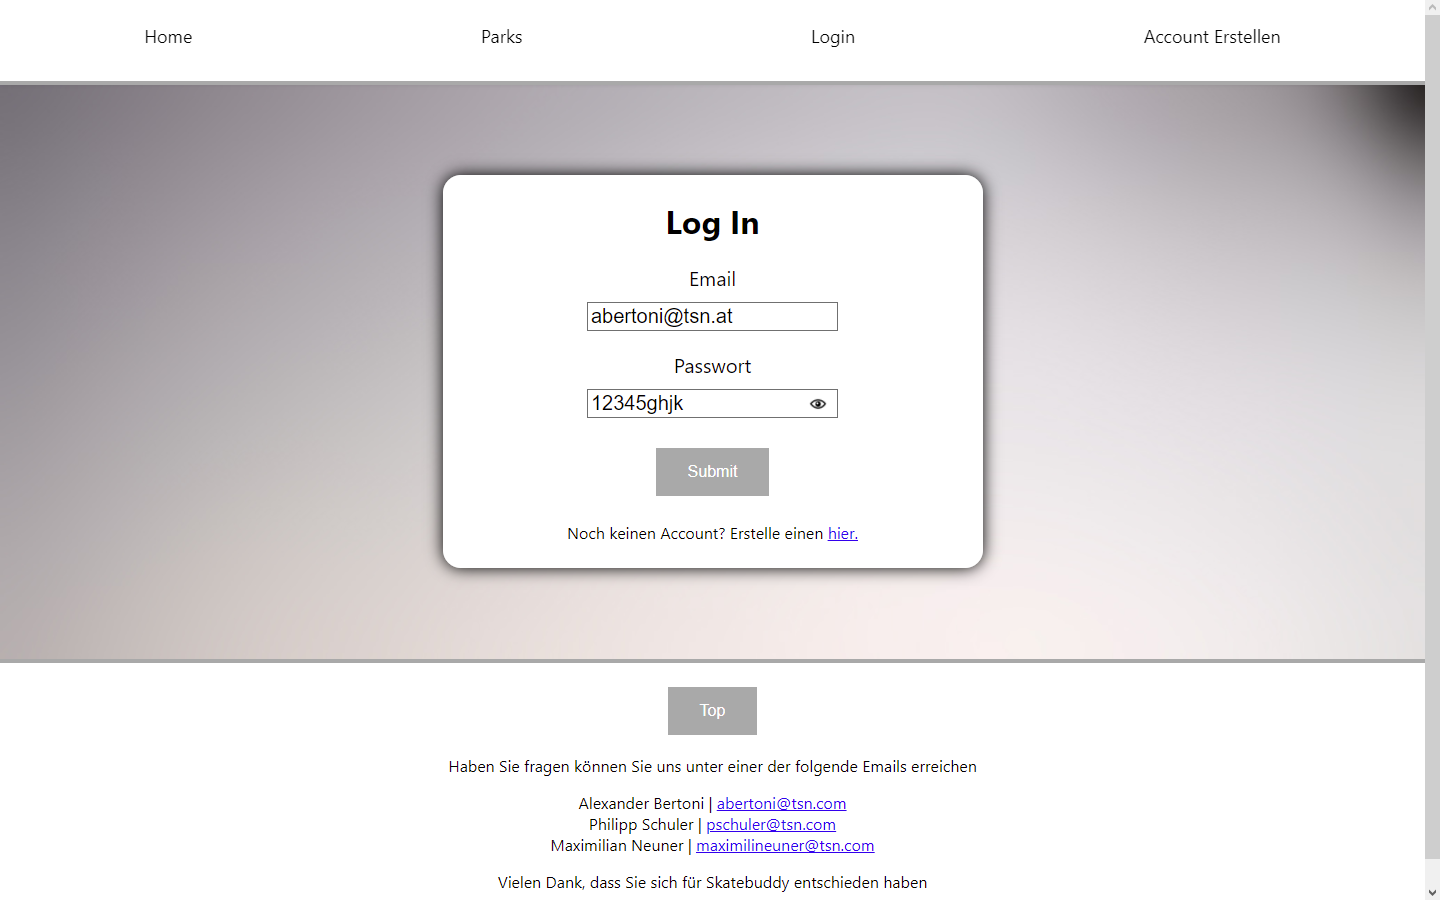
\includegraphics[width=1\textwidth]{Website/LogIn-Passwort-anzeigen.png}}
      \caption{Login Page mit gezeigtem Passwort}
    \end{center}
\end{figure}

\subsection{Augensymbol}
\begin{code}[htp]
\begin{lstlisting}
    .toggle-button {
        margin-top: 0;
        margin-left: -30px;
        height: 17px;
        width: 20px;
        border: white;
        background: no-repeat url('./eye.png');
        background-size: cover;
        cursor: pointer;
    }
\end{lstlisting}
\caption{CSS -  CSS des Augensymbols}
\end{code}
\begin{code}[htp]
\begin{lstlisting}
    const togglePassword = () =>{
        setPasswordShown(!passwordShown)
    }
\end{lstlisting}
\caption{JavaScript Funktion -  Variablenändern bei Knopfdruck}
\end{code}
\begin{code}[htp]
\begin{lstlisting}
    <input className="input" type={passwordShown ? "text" : "password"} onChange={e => setPassword(e.target.value)} />
    <button type="button" onClick={togglePassword} className="toggle-button"></button>
\end{lstlisting}
\caption{HTML - Input und Knopf für Passwort anzeigen}
\end{code}

\begin{figure}[H]
    \begin{center}
      \frame{
\includegraphics[width=0.2\textwidth]{Website/eye.png}}
      \caption{Augensymbol zum Umschalten}
    \end{center}
\end{figure}

Das Auge ist ein einfacher Knopf mit einem Bild als Hintergrund, welcher mit einer JavaScript Funktion 
eine Variable auf true setzt. Ist diese Variable auf \textit{true} wird der Input-Type des inputs von
\textit{password} auf \textit{text} umgeschaltet und das Passwort somit sichtbar. 
